\articlehead{Species Selection and Character Creation: Follow-Up}{Makyo}{2013}

This is just a quick follow-up with some further information about the Species Selection and Character Creation article posted last week.  I normally post on Wednesdays and I had an article that could have been scheduled today, but with that article likely needing more space than this one and the desire not to distract from it with a simple addendum, I figured I'd swap the two days around and give tomorrow's real article its time as the featured post!

Last Wednesday, even as the article was going live, I was packing up my laptop for an afternoon at a coffee shop (The Alley Cat, where the phone is always answered with a personable ``meow!'') where I would spend a few hours talking with the inimitable Klisoura about furries and data.  Among other topics (some of which will show up here on [a][s] quite soon), we poked around some of the species data a little further, and found some more interesting facts.  That, combined with some input from others both on Twitter and FurAffinity, and some volunteers in private communication, got me thinking that more information is always better than less, and so here we go!

\subsection*{Common Terms}

Over the process of exploring the data with Klisoura, we removed several common words such as the name of the species, articles such as `a' or `an', and so on.  However, we left in many additional terms that showed variation between species as they do help show the differences in the ways in which people thought of their characters.  A few of these words, such as `love'/'loved' or `personality' show up on every chart, of course, but at different rates, showing a stronger sense of, say, personality alignment with one species, but with a greater sense of, say, loving with another species.

However, this tends to hide some of the differences in responses that show species perception rather than character perception due to their relative prevalence.  By removing these common words as well, we find that the words associated with the stereotypes or perception of a particular species are emphasized even further, and those differences made plain.  Check it out below!

\begin{figure}
  \begin{center}
    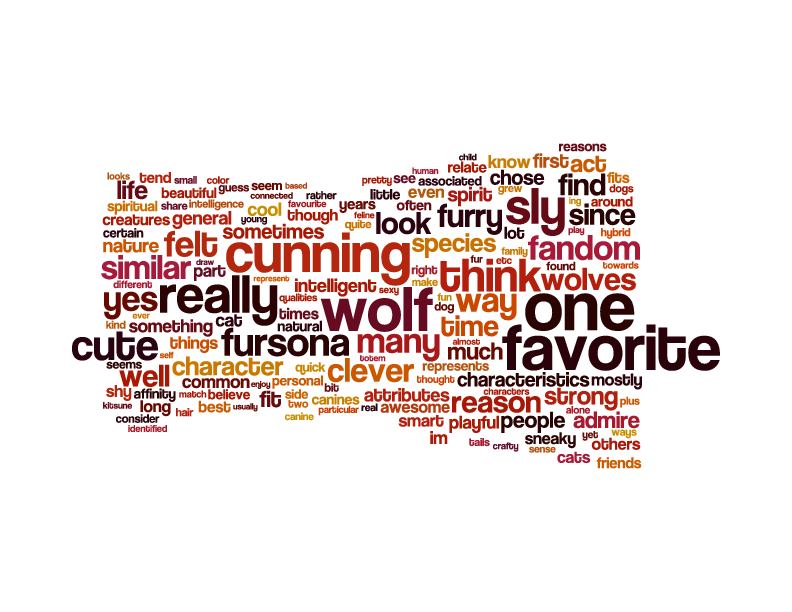
\includegraphics[width=\textwidth]{content/assets/species-2--redfox}
  \end{center}
  \caption{Red Foxes}
\end{figure}

\begin{figure}
  \begin{center}
    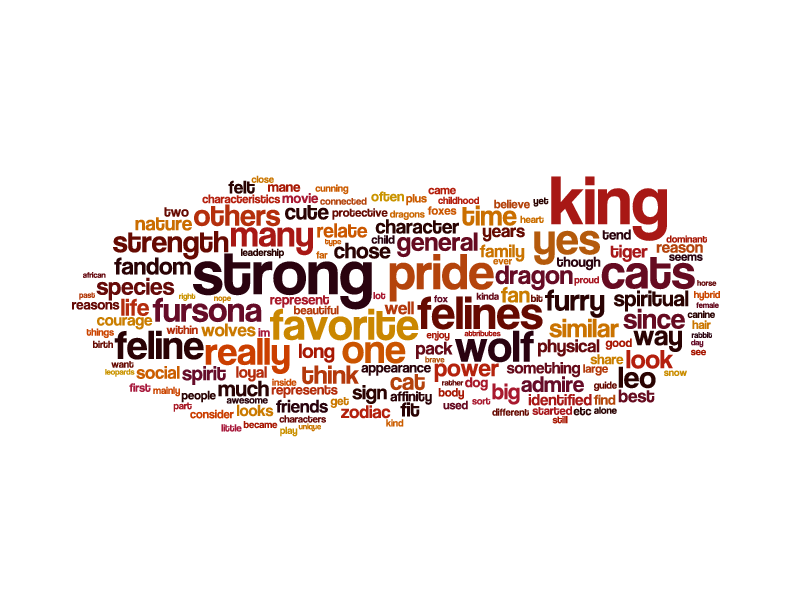
\includegraphics[width=\textwidth]{content/assets/species-2--lion}
  \end{center}
  \caption{Lions}
\end{figure}

\begin{figure}
  \begin{center}
    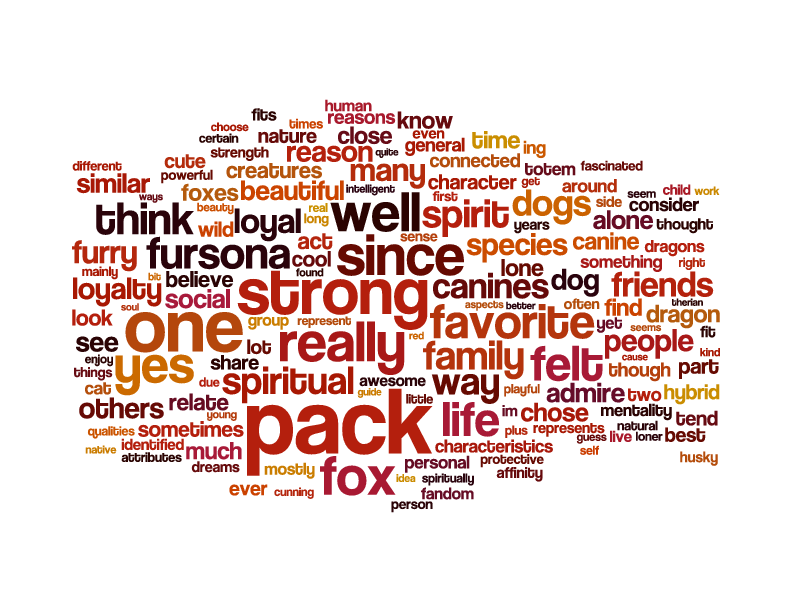
\includegraphics[width=\textwidth]{content/assets/species-2--wolf}
  \end{center}
  \caption{Wolves}
\end{figure}

\begin{figure}
  \begin{center}
    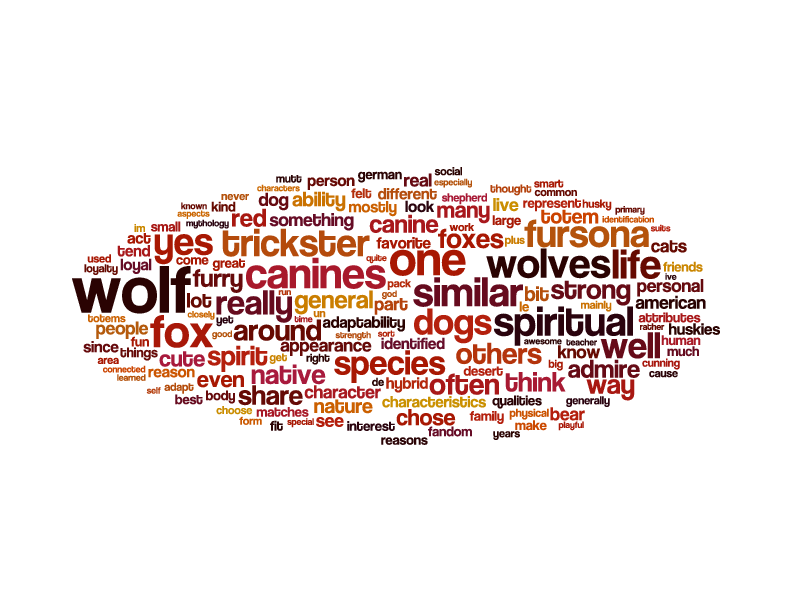
\includegraphics[width=\textwidth]{content/assets/species-2--coyote}
  \end{center}
  \caption{Coyotes}
\end{figure}

\begin{figure}
  \begin{center}
    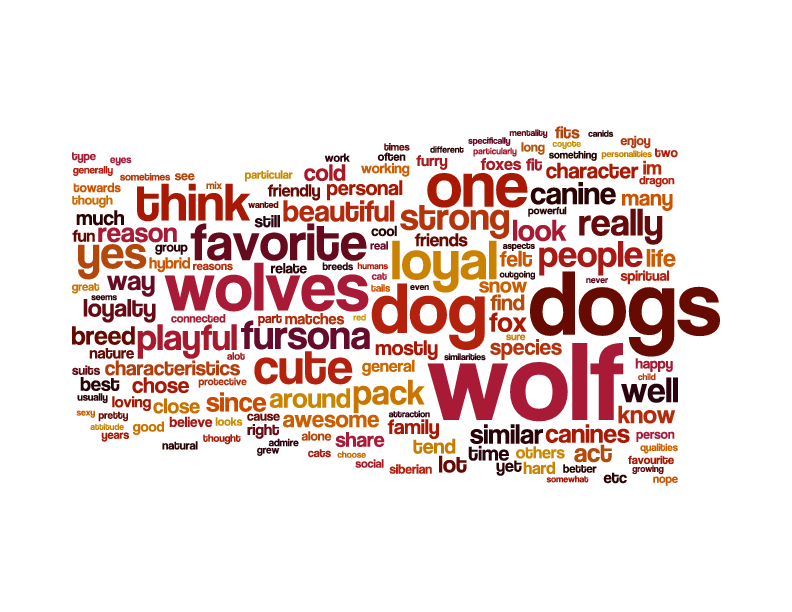
\includegraphics[width=\textwidth]{content/assets/species-2--husky}
  \end{center}
  \caption{Huskies}
\end{figure}

\begin{figure}
  \begin{center}
    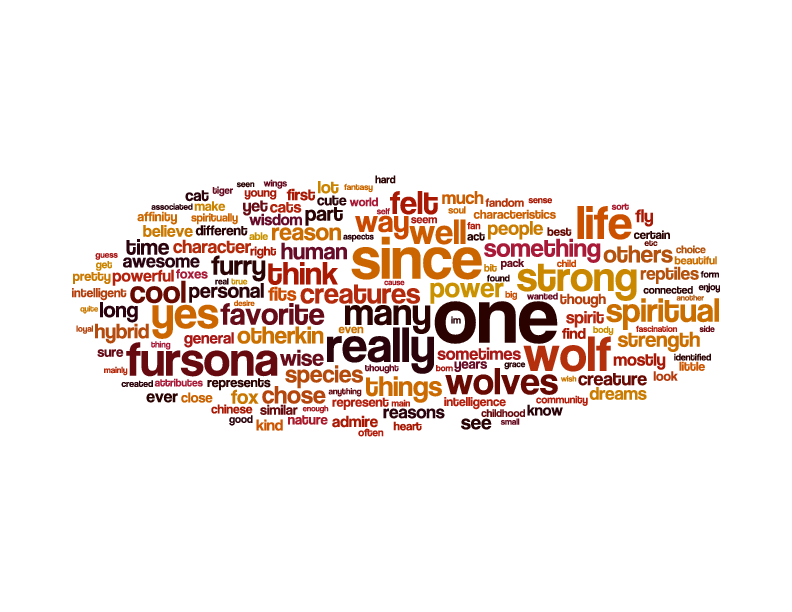
\includegraphics[width=\textwidth]{content/assets/species-2--dragon}
  \end{center}
  \caption{Dragons}
\end{figure}

\begin{figure}
  \begin{center}
    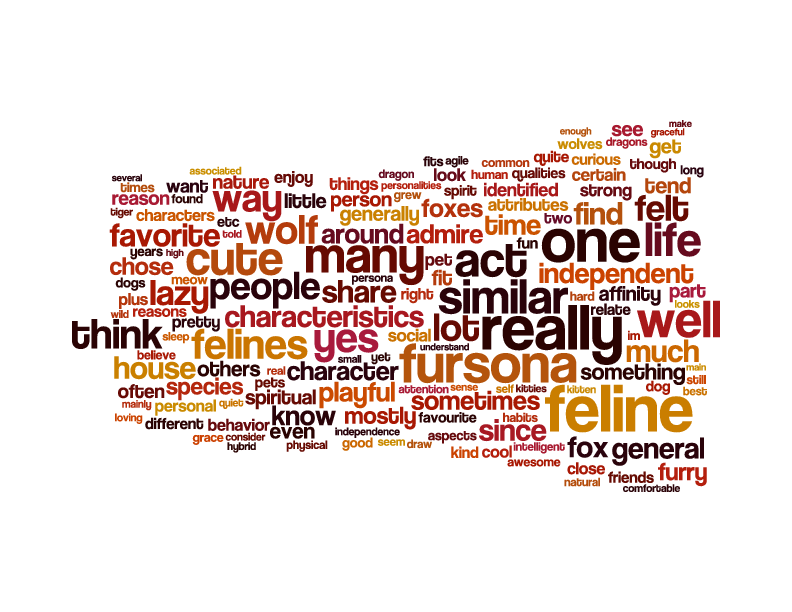
\includegraphics[width=\textwidth]{content/assets/species-2--cat}
  \end{center}
  \caption{Domestic Cats}
\end{figure}

\begin{figure}
  \begin{center}
    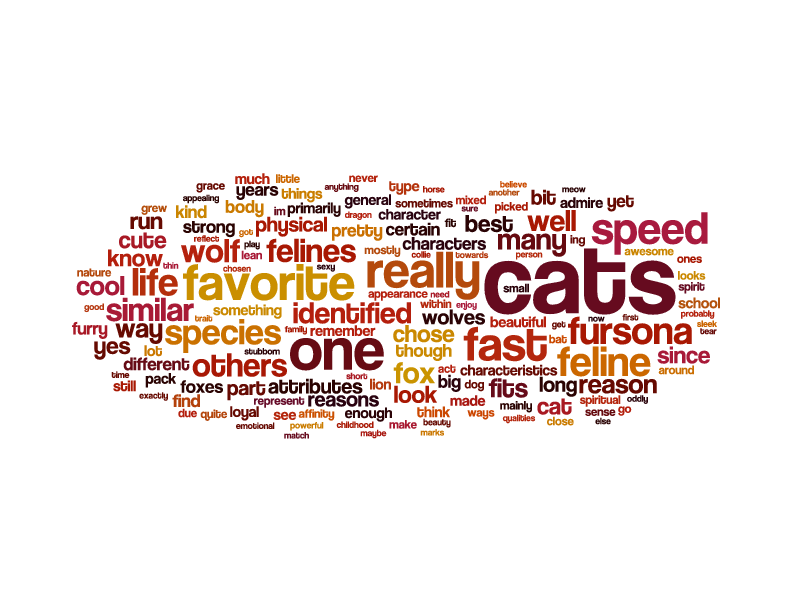
\includegraphics[width=\textwidth]{content/assets/species-2--cheetah}
  \end{center}
  \caption{Cheetahs}
\end{figure}

\begin{figure}
  \begin{center}
    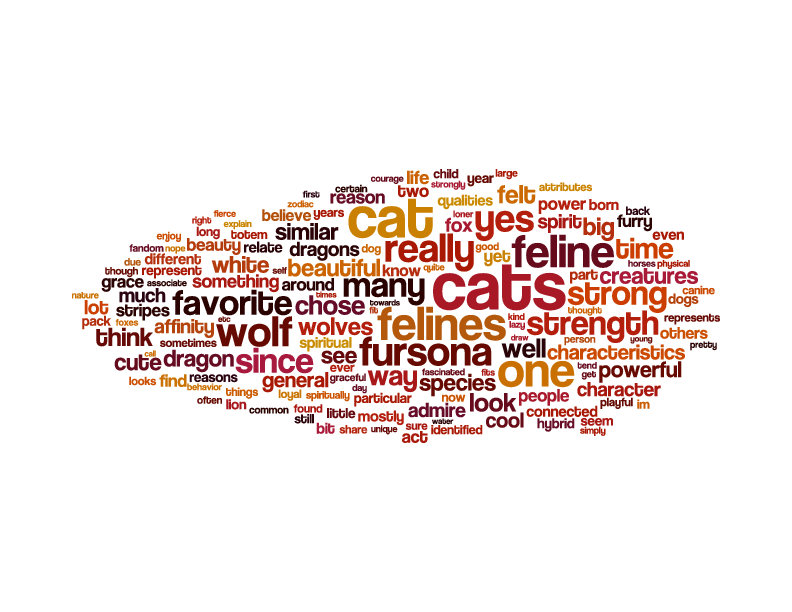
\includegraphics[width=\textwidth]{content/assets/species-2--tiger}
  \end{center}
  \caption{Tigers}
\end{figure}

\begin{figure}
  \begin{center}
    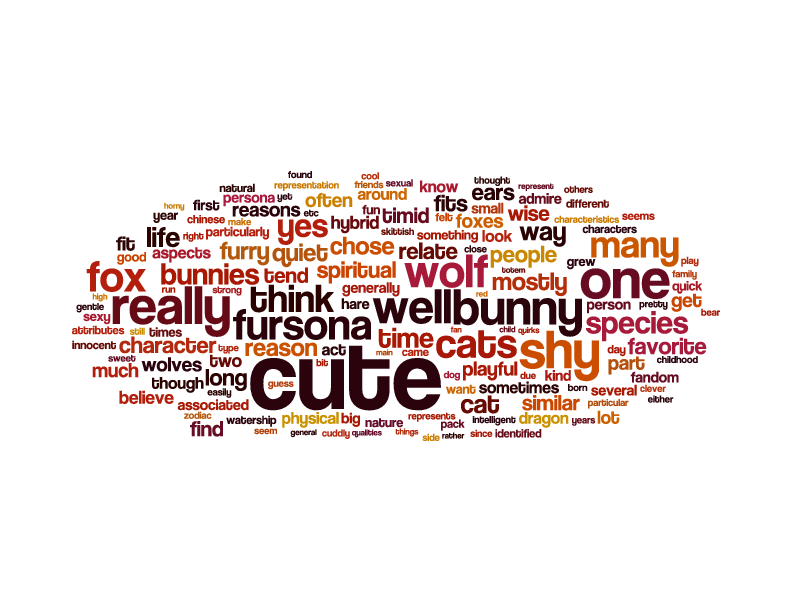
\includegraphics[width=\textwidth]{content/assets/species-2--rabbit}
  \end{center}
  \caption{Rabbits}
\end{figure}

\subsection*{Additional Surveys, Visualization, and Exploration}

The amount of data amassed is quite large.  Current data sets include the Furry Survey from 2009 until present (though we will not be providing information from current data until the 2013 survey itself is finished), the 2012 [adjective][species] Census and Survey, and all of the [a][s] small polls and surveys, not to mention aggregated data from other sources such as the IARP and other surveys, and scrape-able data-sources which we have used in the past.

As I am fond of saying in the Exploring the Fandom Through Data panel*, exploration is a cycle of sorts: from collection of data through understanding, giving back, dialog, and back to data collection.  This is a big portion of that cycle.  When we pull together data from the various sources, that's a big part of the understanding stop of that cycle, just as presenting visualizations such as the word-clouds is a big part of the giving back portion.  By presenting this data in a form that shows some of the story behind it, we can start a dialog between those who produce the results and those who consume them, which leads right back to the beginning: collection.  This, of course, is a fancy way of saying, we invite comments and questions by posting these results freely.  More than that, we love the feedback, because that's what helps drive us to ask new questions, explore new topics, and try to understand more of our subculture.

We got several responses to the last post, and I think it would be good to expose some of this process to all so that we can see what goes on in this whole cycle.

\begin{description}
  \item[I'd like to see X species/Why didn't you do X?] We have data for several species, plus several write-in answers for additional species that were not available through the check-boxes.  However, as the number of respondents nears one for each given species, two things can happen to the data: it can either get skewed wildly in inappropriate directions, or it can near the normal distribution of words within any given text.  For example, if we were to take this here paragraph, we'd see a fairly normal distribution of words, with a slightly higher weight on `species', but nothing out of the norm.  However, if you were to respond to your choice of species of ``fox'' with ``fox fox fox fOX FOX FOX OH MAN I LOVE FOXES'', then, as you can see, the distribution is wildly skewed toward `fox'.  This was the reason for us restricting data to the more popular species responses out there: we are more likely to see trends that might, in some way, represent those who respond with a given answer.
  \item[This totally jives with why I chose X/I can't understand why people would answer in such a way!] First of all, these are only general trends that express the reasons for choosing a species to represent oneself.  The are hardly guides, and they often fall along social perceptions of the species in wider culture, outside of furry (thinking of wolves in a pack, speedy cheetahs, or cunning foxes is hardly out of the norm for western society).  Secondly, did you take the Furry Survey? If something seems missing, it could be your response!
  \item[What about fandom perceptions that make species more appealing?] I mentioned in last week's article that there were what I termed ``self-reinforcing stereotypes'' associated with many species.  For instance, Altivo mentions those who would choose fox, husky, or horse due solely for their perceived sexual role within the fandom.  This is most assuredly worth an article of its own, but in brief, that is a difficult thing to measure both in the data as explored and also in the responses to the questions asked at the Species Selection and Character Creation panel.  Needless to say, we haven't forgotten about fandom-specific stereotypes as a factor in selection, simply that the point of the article was to explore selection as a more general topic.
  \item[Have you tried correlating against X?/What further things can be done with the data?] This sentiment is perhaps best expressed by FA user NEXRAD in their comments on the Jackals/Coyotes post on FA.  There is a lot -- a lot -- of data in all of the responses to the Furry Survey.  In fact there are a stupefying number of data points in any one year of the survey!  We can look for trends, such as we have done with the species, or model relationships based on correlations or clustering as was suggested.  All of these are possible, but they take time and we are, for the most part, lay-critters doing the best we can outside our day jobs, and checking our work before sending it out into the world.  (Additionally, [a][s] has some restrictions that prevented the topic from being explored further in last week's article: we try to keep our articles at about 2,000 words or under to help with readability and comprehension, and so the best place for such work is in future articles, posts, and visualizations!)
\end{description}

Finally, we'd like to reiterate the sentiment that has been in place with the Furry Survey for several years now.  We do our best to present a fairly solid breakdown of the information provided in the surveys, but we welcome requests for larger data sets from other researchers in the future.  These aren't available for direct download currently, and will take some time to anonymize and prepare, but they do exist, and the same holds true as with ``more information'': more eyes on that information is always better!

* Which, if everything works out okay, I should be able to provide as an updated recording soon.  We have video and audio recordings from RMFC this year, and if their quality is good enough, we'll pull them together and put them up on Vimeo as we did last year.
